\documentclass[conference]{IEEEtran}

\usepackage[T1]{fontenc}
\usepackage[utf8]{inputenc}
\usepackage{amsmath,amssymb}
\usepackage{graphicx}
\usepackage{booktabs}
\usepackage{array}
\usepackage{url}
\usepackage[colorlinks=true,linkcolor=blue,citecolor=blue,urlcolor=blue]{hyperref}
\usepackage{microtype}
\usepackage{balance}

\graphicspath{{figures/}{images/}}
\newcommand{\Rsq}{$R^{2}$}

\begin{document}

\title{Supervised Learning for WHOOP Fitness Recovery Score Prediction}

\author{\IEEEauthorblockN{Yash David Bedekar}
\IEEEauthorblockA{\textit{MSc Data Science} \\
\textit{University of Europe for Applied Sciences} \\
Potsdam, Germany \\
yash.bedekar@ue-germany.de}
\and
\IEEEauthorblockN{Raja Hashim Ali}
\IEEEauthorblockA{\textit{Department of Business} \\
\textit{University of Europe for Applied Sciences} \\
Potsdam, Germany \\
hashim.ali@ue-germany.de}}

\maketitle

\begin{abstract}
In this report, I present my supervised learning project on predicting WHOOP recovery scores from wearable fitness data. I used a dataset with 100{,}000 daily records and compared multiple regression models, including linear, regularized, tree-based, and boosting approaches. The project was designed to answer not only which model performs best, but also how preprocessing affects performance, which features are most important, and how robust the best model is when data quality becomes worse. The results show that Linear Regression gave the strongest overall performance, with cross-validated \Rsq{} of 0.446, MAE of 10.53, and RMSE of 13.14. Resting heart rate, HRV, and their baseline values were the most influential predictors across the analysis. I also found that the model remains reasonably stable when small noise is added, but performance drops strongly when important inputs are missing.
\end{abstract}

\begin{IEEEkeywords}
supervised learning, regression, wearable analytics, recovery prediction, WHOOP, HRV
\end{IEEEkeywords}

\section{Introduction}
The goal of this project is to predict the daily \texttt{recovery\_score} using wearable and profile data from the WHOOP Fitness Dataset. Recovery score is useful because it gives a simple summary of how ready a person may be for training, physical activity, or general recovery. In practice, this kind of score can help support daily decisions by translating many physiological signals into one easy value.

In this project, I applied supervised learning to compare different regression models and identify which one gives the best balance between prediction quality, simplicity, and practical use. I did not want to focus only on accuracy. I also wanted to understand how the models behave, which features matter the most, and whether the best model would still be reliable when the data is noisy or incomplete.

This report is fully based on the outputs generated by my implemented code. All tables and figures included here come from the project result files, which helps keep the report consistent with the code, results, and saved outputs.

\section{Related Work / Background}
Wearable devices are now widely used to track health and fitness signals such as heart rate, heart rate variability (HRV), sleep, activity strain, and recovery. Research on athlete monitoring shows that recovery is influenced by a combination of physiological and behavioral signals rather than by a single measurement alone. In particular, HRV and resting heart rate are often used as useful indicators of fatigue, stress, and readiness \cite{plews2013heart,bellenger2016monitoring}.

Commercial platforms such as WHOOP combine multiple inputs, including HRV, resting heart rate, sleep, and strain, into a single recovery score \cite{whoop2023methodology}. Even though the exact proprietary calculation is not fully public, the general idea is clear: recovery should reflect the combined effect of cardiovascular state, sleep quality, and physical load. This makes the problem suitable for supervised learning, especially when many input variables are available.

From a machine learning perspective, this is a structured tabular prediction problem. For this type of data, both simple linear models and more complex ensemble methods are commonly used \cite{sklearn,chen2016xgboost}. However, more complex models do not always perform better. When the predictive signal is spread across many weak features and the overall relationships are mostly additive, linear models can generalize well and remain much easier to interpret. This idea is important for my project because the best model should not only be accurate, but also practical and explainable.

\section{Dataset Description}
The dataset used in this project is the WHOOP Fitness Dataset from Kaggle \cite{kaggle_whoop}. It contains 100{,}000 daily records with 41 input features and one target variable, \texttt{recovery\_score}. To keep the experiments manageable and reproducible, I sampled 30{,}000 rows from the full dataset using random seed 42.

\begin{table}[htbp]
\caption{Project Dataset Summary}
\label{tab:data_summary}
\centering
\begin{tabular}{ll}
\toprule
\textbf{Item} & \textbf{Value} \\
\midrule
Dataset & WHOOP Fitness Dataset \\
Source & Kaggle \\
Full size & 100{,}000 rows \\
Rows used in project & 30{,}000 \\
Input features & 41 \\
Target & \texttt{recovery\_score} \\
Target range & 0 to 100 \\
Train-test split & 80\% / 20\% \\
Validation & 5-fold cross-validation \\
\bottomrule
\end{tabular}
\end{table}

The input variables can be grouped into a few broad categories. The first group contains cardiovascular variables such as HRV, resting heart rate, average heart rate, and their baseline values. The second group contains sleep-related variables such as sleep duration, sleep efficiency, deep sleep, light sleep, and REM sleep. A third group describes activity and strain, including calories burned, activity duration, and heart-rate zone measures. The final group contains user profile and temporal variables such as age, fitness level, sport type, and date-related features.

The target variable is the daily \texttt{recovery\_score}, which is a continuous value between 0 and 100. This makes the task a standard supervised regression problem.

\section{Problem Statement}
This project is a supervised regression task. Each daily record is represented by a feature vector $\mathbf{x} \in \mathbb{R}^{d}$, and the goal is to predict a continuous target value $y$, where $y$ is the recovery score.

\begin{equation}
\hat{y} = \hat{f}(\mathbf{x}) \approx y, \qquad y \in [0,100]
\end{equation}

The objective is to learn a model $\hat{f}$ that predicts the recovery score as accurately as possible from the available daily inputs. I evaluated model performance using three common regression metrics:
\begin{itemize}
  \item Mean Absolute Error (MAE)
  \item Root Mean Squared Error (RMSE)
  \item Coefficient of determination (\Rsq{})
\end{itemize}

These metrics allow me to compare not only the average size of the prediction errors, but also how much variance in the recovery score the model is able to explain.

\section{Research Questions}
To keep the analysis structured, I organized the project around seven research questions that match the outputs generated by my code.

\begin{itemize}
  \item \textbf{RQ1:} How well do basic regression models perform in predicting WHOOP recovery score?
  \item \textbf{RQ2:} Which model performs best overall, and do ensemble methods improve on simple baselines?
  \item \textbf{RQ3:} How much does preprocessing affect model performance?
  \item \textbf{RQ4:} Which features are the most important for prediction?
  \item \textbf{RQ5:} Are the model rankings stable across different evaluation metrics?
  \item \textbf{RQ6:} How robust is the best model under noisy and incomplete data?
  \item \textbf{RQ7:} Which model is the best practical recommendation when accuracy and usability are considered together?
\end{itemize}

\section{Methodology}
My workflow followed a standard supervised learning pipeline. I first loaded the dataset, converted the date column into useful calendar-based features, removed identifiers, and separated the target variable from the inputs. I then compared multiple preprocessing strategies and several regression models.

\subsection{Data Preparation}
The preprocessing workflow included missing-value imputation, optional feature scaling, and one-hot encoding for categorical fields. The goal was to compare both simple and more complete preprocessing pipelines rather than assuming that a more complicated pipeline would automatically perform better.

Three preprocessing settings were compared:
\begin{itemize}
  \item Numeric-only features with median imputation
  \item Numeric features with median imputation and scaling
  \item Full pipeline with scaling and categorical encoding
\end{itemize}

\subsection{Models}
The tested models were Linear Regression, Ridge Regression, Elastic Net, Decision Tree, Random Forest, Gradient Boosting, and XGBoost. These models were chosen because they cover a useful range from very simple baselines to stronger non-linear ensemble methods.

\subsection{Evaluation}
I used both hold-out testing and cross-validation. The hold-out split was mainly used for direct comparison tables and visual diagnostics. Five-fold cross-validation was used to obtain more stable performance estimates and to compare ranking consistency across models.

The main evaluation metrics were:
\begin{equation}
\mathrm{MAE} = \frac{1}{n}\sum_{i=1}^{n}|y_i-\hat{y}_i|
\end{equation}

\begin{equation}
\mathrm{RMSE} = \sqrt{\frac{1}{n}\sum_{i=1}^{n}(y_i-\hat{y}_i)^2}
\end{equation}

\begin{equation}
R^2 = 1 - \frac{\sum_{i=1}^{n}(y_i-\hat{y}_i)^2}{\sum_{i=1}^{n}(y_i-\bar{y})^2}
\end{equation}

\subsection{Explainability and Robustness}
To understand model behavior, I studied feature importance using two approaches: aggregated tree-based importance and permutation importance. This helped me check whether the same features remained important across different methods.

To test robustness, I evaluated the best model under three conditions: clean data, added numeric noise, and simulated missingness. This part of the project was important because a useful model should still behave reasonably when real-world data quality is not perfect.

\begin{figure}[htbp]
  \centering
  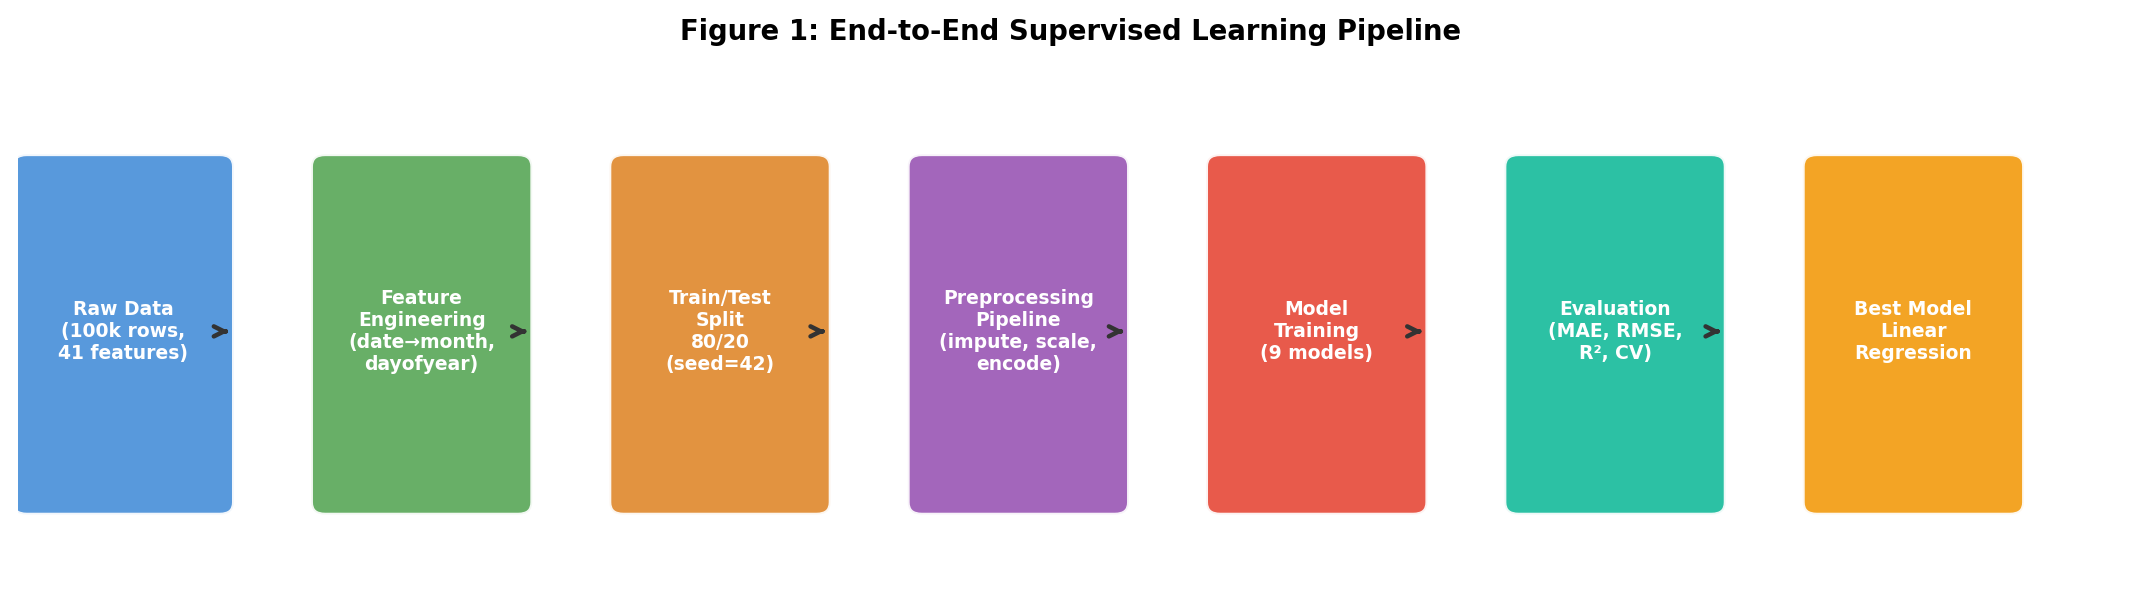
\includegraphics[width=\linewidth]{DIAG_pipeline.png}
  \caption{Pipeline used in the project from preprocessing to model selection.}
  \label{fig:pipeline}
\end{figure}

\section{Experimental Setup}
All experiments were run in Python using the implemented machine learning pipeline. I used a fixed random seed of 42 for sampling, splitting, and validation so that the results could be reproduced. The 30{,}000-row project sample was divided into an 80/20 train-test split, and 5-fold cross-validation was used for more stable model comparison.

\begin{table}[htbp]
\caption{Software and Evaluation Setup}
\label{tab:setup}
\centering
\begin{tabular}{ll}
\toprule
\textbf{Component} & \textbf{Detail} \\
\midrule
Language & Python 3.x \\
Libraries & pandas, NumPy, scikit-learn, XGBoost \\
Random seed & 42 \\
Sample size & 30{,}000 rows \\
Hold-out set & 6{,}000 rows \\
Validation & 5-fold cross-validation \\
Outputs saved as & CSV tables and PNG figures \\
\bottomrule
\end{tabular}
\end{table}

The project outputs were saved automatically into the \texttt{outputs/tables} and \texttt{outputs/figures/images} folders. The report uses these generated files as the source for the presented tables, figures, and numeric summaries.

\section{Results and Discussion}
\subsection{RQ1: Baseline Performance}
I started by testing a small set of basic models to understand how difficult the prediction problem is. The baseline comparison included Linear Regression, Decision Tree, and k-Nearest Neighbours.

\begin{table}[htbp]
\caption{RQ1 Baseline Hold-out Performance}
\label{tab:rq1}
\centering
\begin{tabular}{lccc}
\toprule
\textbf{Model} & \textbf{MAE} & \textbf{RMSE} & \textbf{\Rsq} \\
\midrule
Linear Regression & 10.54 & 13.18 & 0.442 \\
Decision Tree     & 12.75 & 15.91 & 0.187 \\
k-NN              & 13.04 & 16.09 & 0.168 \\
\bottomrule
\end{tabular}
\end{table}

Even in this simple comparison, Linear Regression already performed much better than the other two models. This was an early sign that the dataset may not require a complex non-linear model to capture the main signal.

To understand why the task is challenging, I also looked at the strongest direct correlations between numeric features and the target.

\begin{table}[htbp]
\caption{Top Numeric Correlations with Recovery Score}
\label{tab:corr}
\centering
\begin{tabular}{lc}
\toprule
\textbf{Feature} & \textbf{Absolute Correlation} \\
\midrule
hrv                    & 0.188 \\
resting\_heart\_rate   & 0.176 \\
hr\_zone\_5\_min       & 0.102 \\
activity\_calories     & 0.097 \\
activity\_strain       & 0.094 \\
hr\_zone\_4\_min       & 0.088 \\
age                    & 0.074 \\
activity\_duration\_min & 0.073 \\
\bottomrule
\end{tabular}
\end{table}

The correlations are relatively low, which suggests that no single feature explains the recovery score on its own. This supports the idea that recovery is driven by a combination of many weak signals rather than one dominant input.

\begin{figure}[htbp]
  \centering
  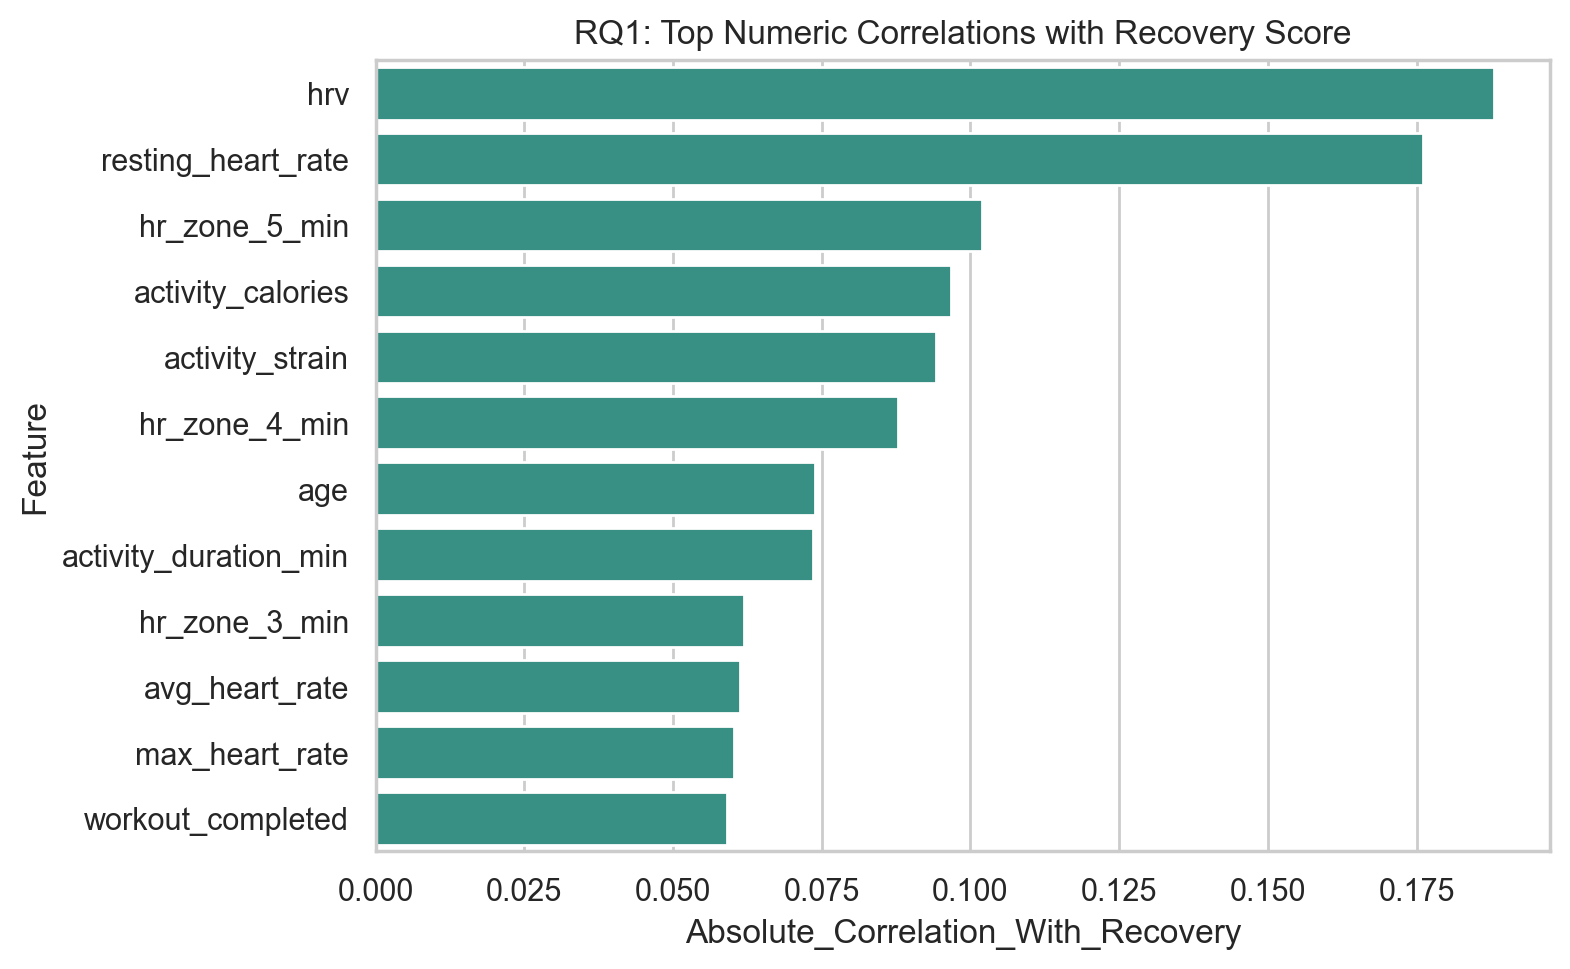
\includegraphics[width=\linewidth]{RQ1_top_numeric_correlations.png}
  \caption{Top absolute numeric correlations with the target variable.}
  \label{fig:rq1corr}
\end{figure}

\subsection{RQ2: Best Performing Model}
After the baseline experiment, I expanded the comparison to the full set of models. The main hold-out results are shown in Table~\ref{tab:model_results}.

\begin{table}[htbp]
\caption{RQ2 Main Model Performance on the Hold-out Set}
\label{tab:model_results}
\centering
\begin{tabular}{lccc}
\toprule
\textbf{Model} & \textbf{MAE} & \textbf{RMSE} & \textbf{\Rsq} \\
\midrule
Linear Regression & 10.54 & 13.18 & 0.442 \\
Ridge Regression  & 10.75 & 13.43 & 0.421 \\
XGBoost           & 11.09 & 13.78 & 0.390 \\
Elastic Net       & 11.09 & 13.80 & 0.388 \\
Random Forest     & 11.31 & 14.07 & 0.364 \\
Gradient Boosting & 11.37 & 14.10 & 0.361 \\
Decision Tree     & 12.60 & 15.76 & 0.201 \\
\bottomrule
\end{tabular}
\end{table}

Linear Regression gave the best result on all three metrics. Ridge Regression came second and stayed close, while XGBoost and the other ensemble methods did not improve the performance. This is an important finding because it shows that more model complexity did not lead to better generalization on this dataset.

This result suggests that the predictive signal is mostly additive and relatively simple. In other words, a transparent linear model was enough to capture the useful patterns better than the heavier ensemble models.

\begin{figure}[htbp]
  \centering
  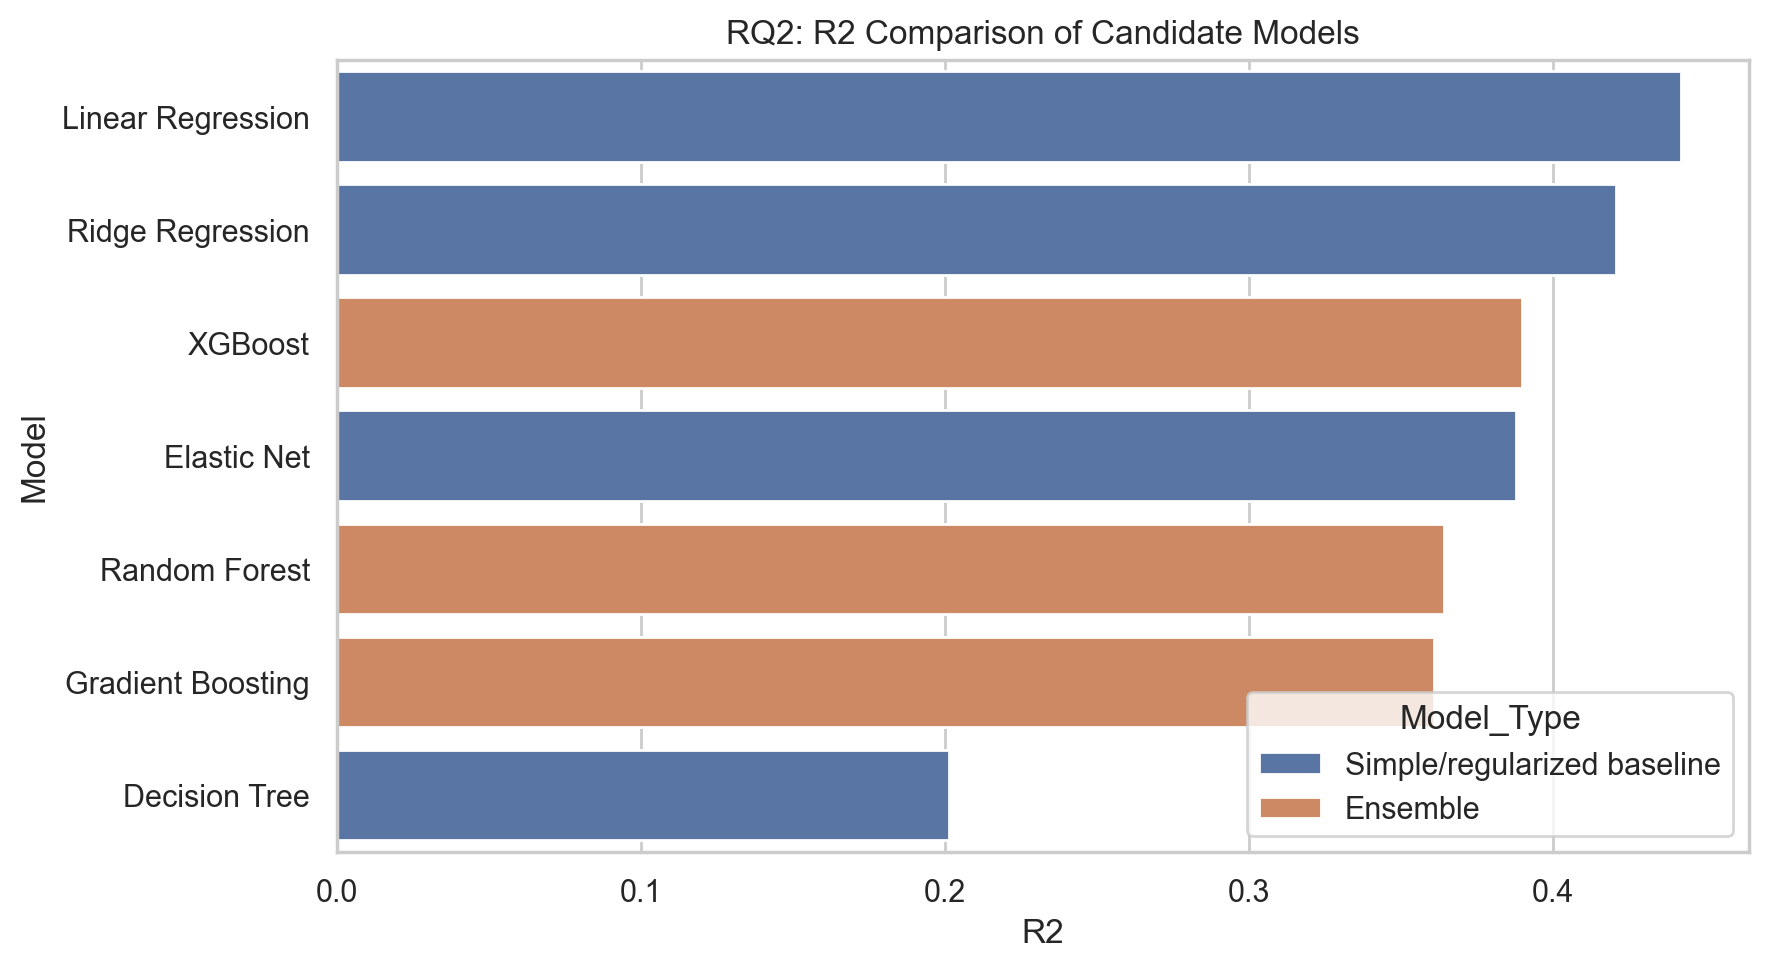
\includegraphics[width=\linewidth]{RQ2_R2_comparison.png}
  \caption{Comparison of \Rsq{} across the tested models.}
  \label{fig:rq2}
\end{figure}

\begin{figure}[htbp]
  \centering
  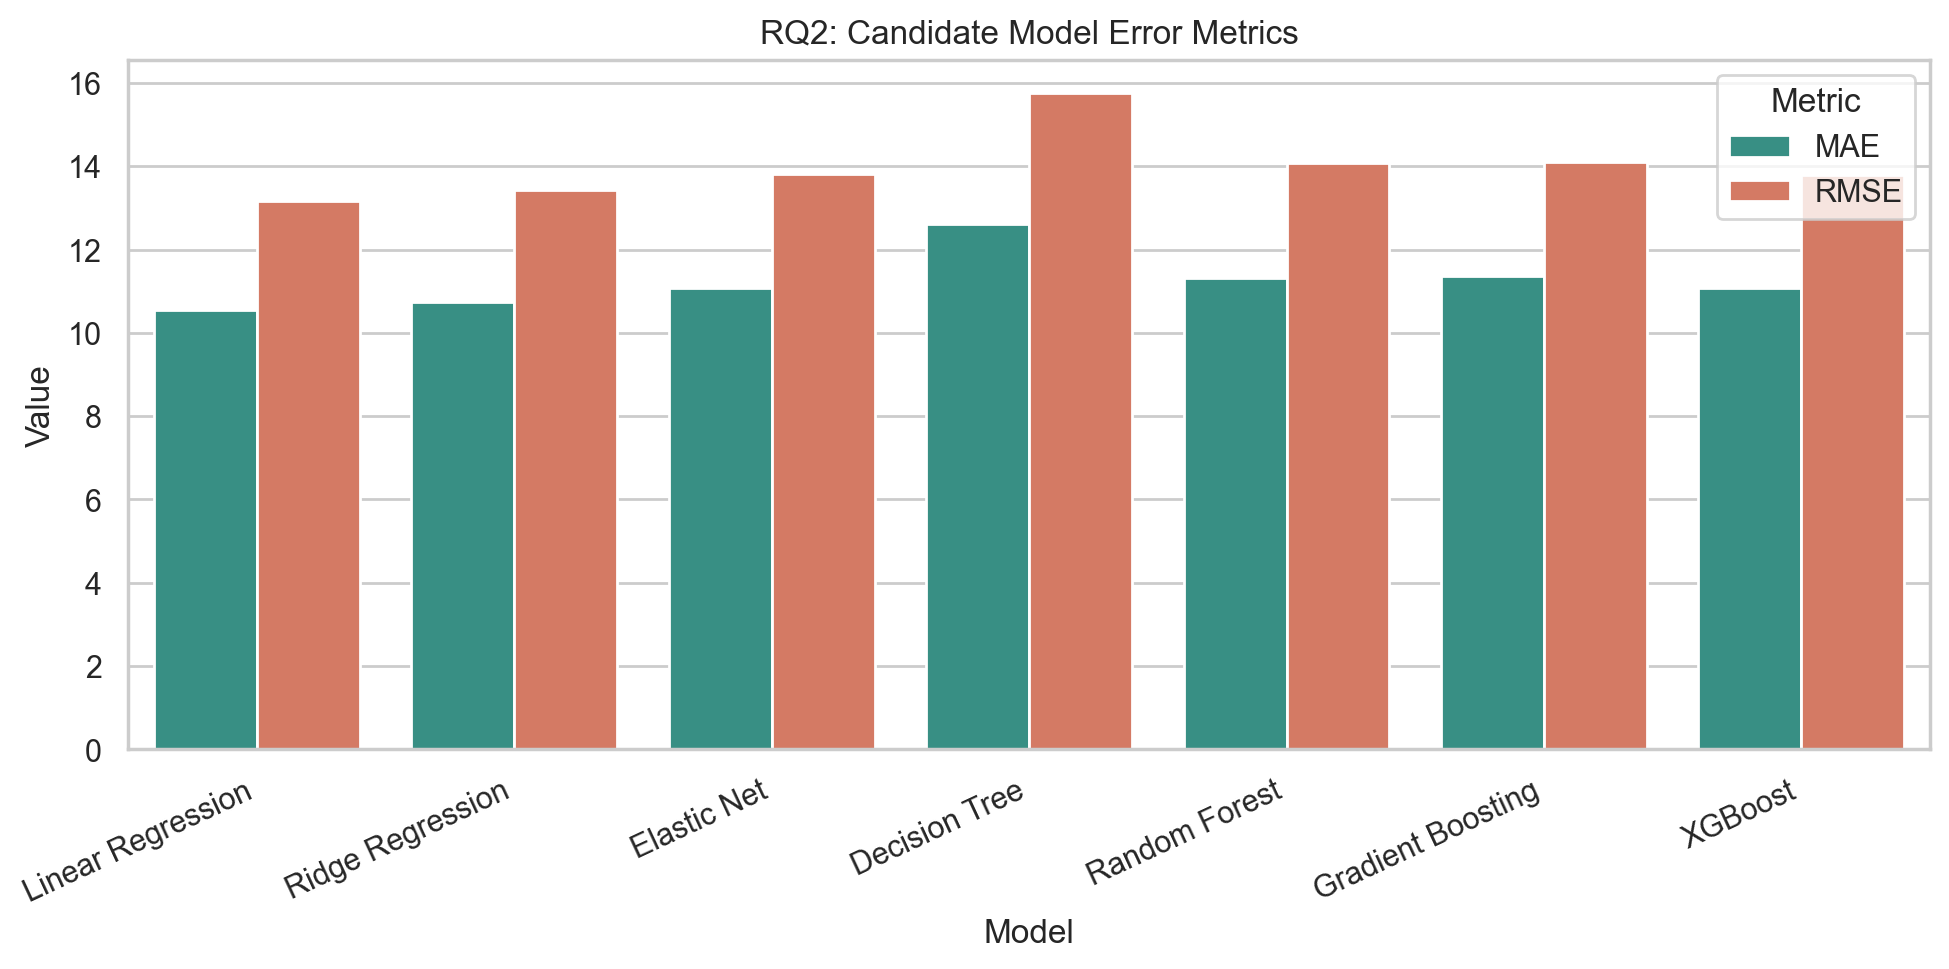
\includegraphics[width=\linewidth]{RQ2_error_metrics.png}
  \caption{Comparison of MAE and RMSE across the tested models.}
  \label{fig:rq2errors}
\end{figure}

\subsection{RQ3: Effect of Preprocessing}
I also checked whether preprocessing had a major effect on the final result. The answer is mostly no. The model performance changed only slightly across the tested pipelines.

\begin{table}[htbp]
\caption{RQ3 Effect of Preprocessing}
\label{tab:preprocessing}
\centering
\begin{tabular}{p{4.2cm}ccc}
\toprule
\textbf{Pipeline} & \textbf{MAE} & \textbf{RMSE} & \textbf{\Rsq} \\
\midrule
Numeric only + imputation & 10.56 & 13.21 & 0.439 \\
Numeric + scaling         & 10.78 & 13.46 & 0.417 \\
Full pipeline + encoding  & 10.75 & 13.43 & 0.421 \\
Full pipeline + Random Forest & 11.31 & 14.07 & 0.364 \\
\bottomrule
\end{tabular}
\end{table}

The best setup was the simpler numeric-only pipeline with median imputation. Adding scaling or a more complete categorical pipeline did not create a meaningful improvement. This tells me that the project does not need a very complicated preprocessing strategy to obtain its strongest result.

\begin{figure}[htbp]
  \centering
  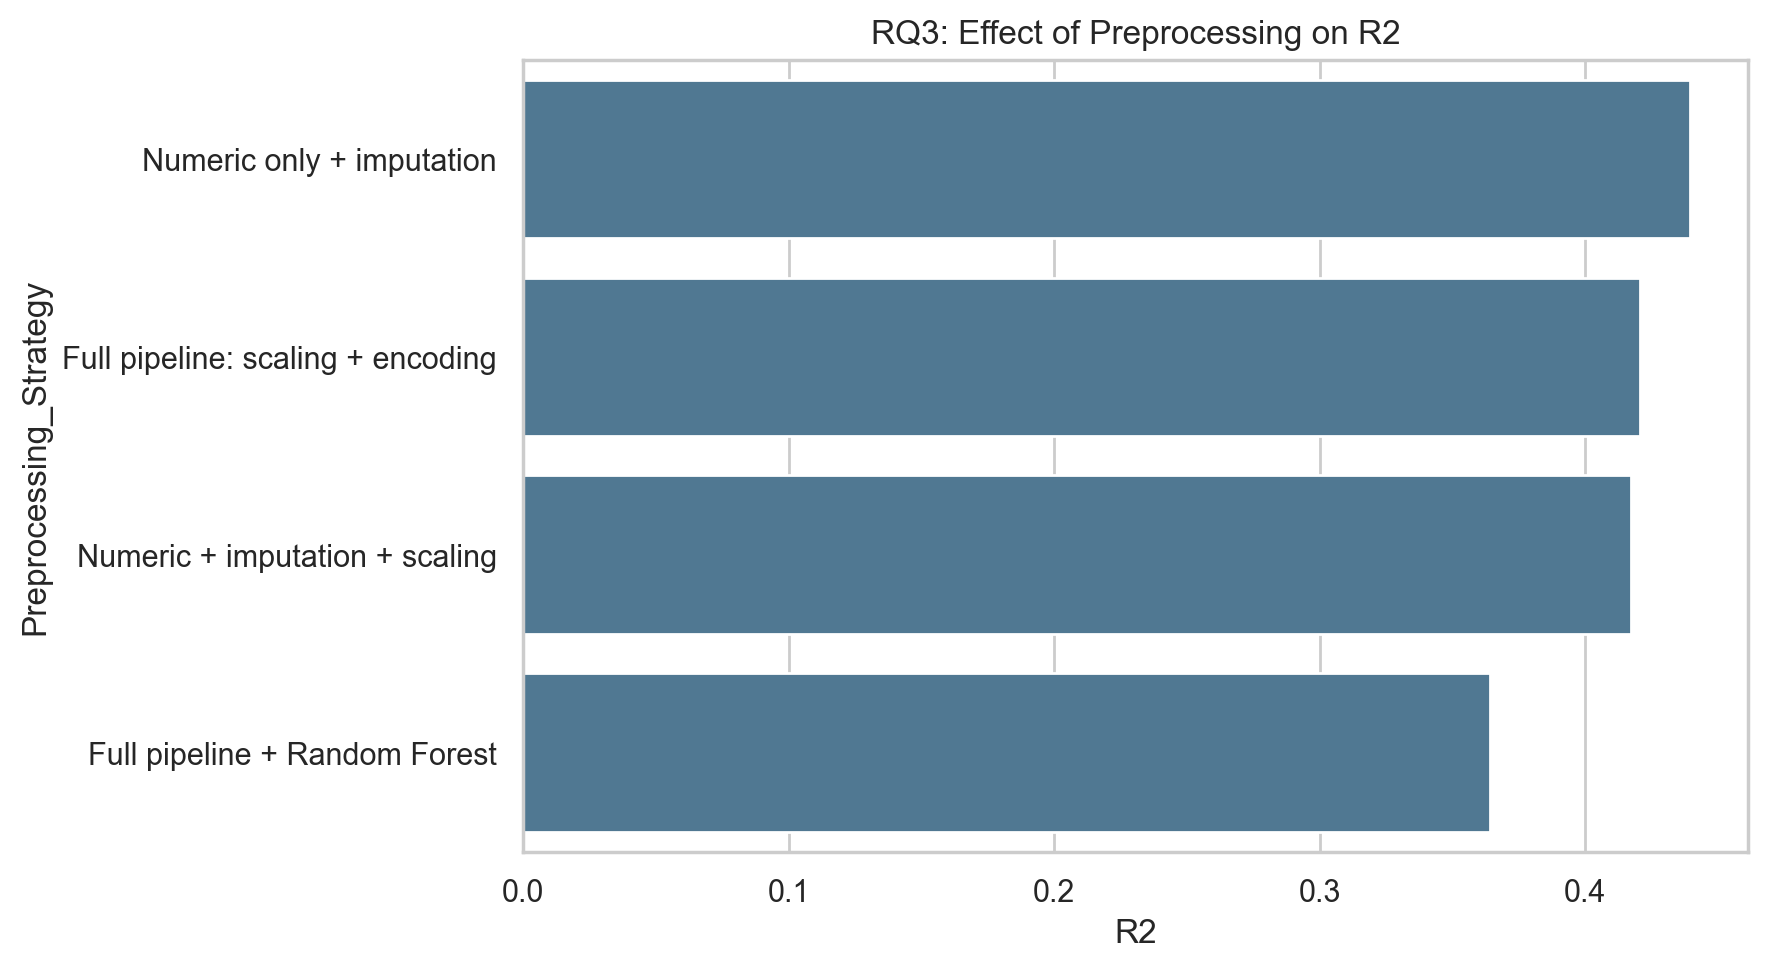
\includegraphics[width=\linewidth]{RQ3_R2_comparison.png}
  \caption{Comparison of \Rsq{} for the tested preprocessing strategies.}
  \label{fig:rq3}
\end{figure}

\subsection{RQ4: Important Features}
Feature importance was one of the most useful parts of the project because it helped explain why the best model works. The strongest predictors came from cardiovascular features. Resting heart rate and HRV clearly mattered the most, followed by their baseline values and daily strain.

\begin{table}[htbp]
\caption{RQ4 Top Features from the Project}
\label{tab:features}
\centering
\begin{tabular}{lcc}
\toprule
\textbf{Feature} & \textbf{Tree Importance (\%)} & \textbf{Permutation $\Delta$\Rsq} \\
\midrule
resting\_heart\_rate & 18.35 & 0.468 \\
hrv                  & 15.98 & 0.275 \\
rhr\_baseline        & 12.83 & 0.378 \\
day\_strain          & 9.99  & 0.114 \\
hrv\_baseline        & 8.66  & 0.162 \\
calories\_burned     & 4.72  & 0.035 \\
date\_dayofyear      & 4.61  & 0.015 \\
age                  & 2.96  & 0.023 \\
\bottomrule
\end{tabular}
\end{table}

The agreement between tree-based importance and permutation importance gives more confidence in these findings. It shows that the model is learning mainly from the same physiological signals across different analysis methods. This is also meaningful from a domain perspective because resting heart rate and HRV are widely associated with recovery and fatigue.

\begin{figure}[htbp]
  \centering
  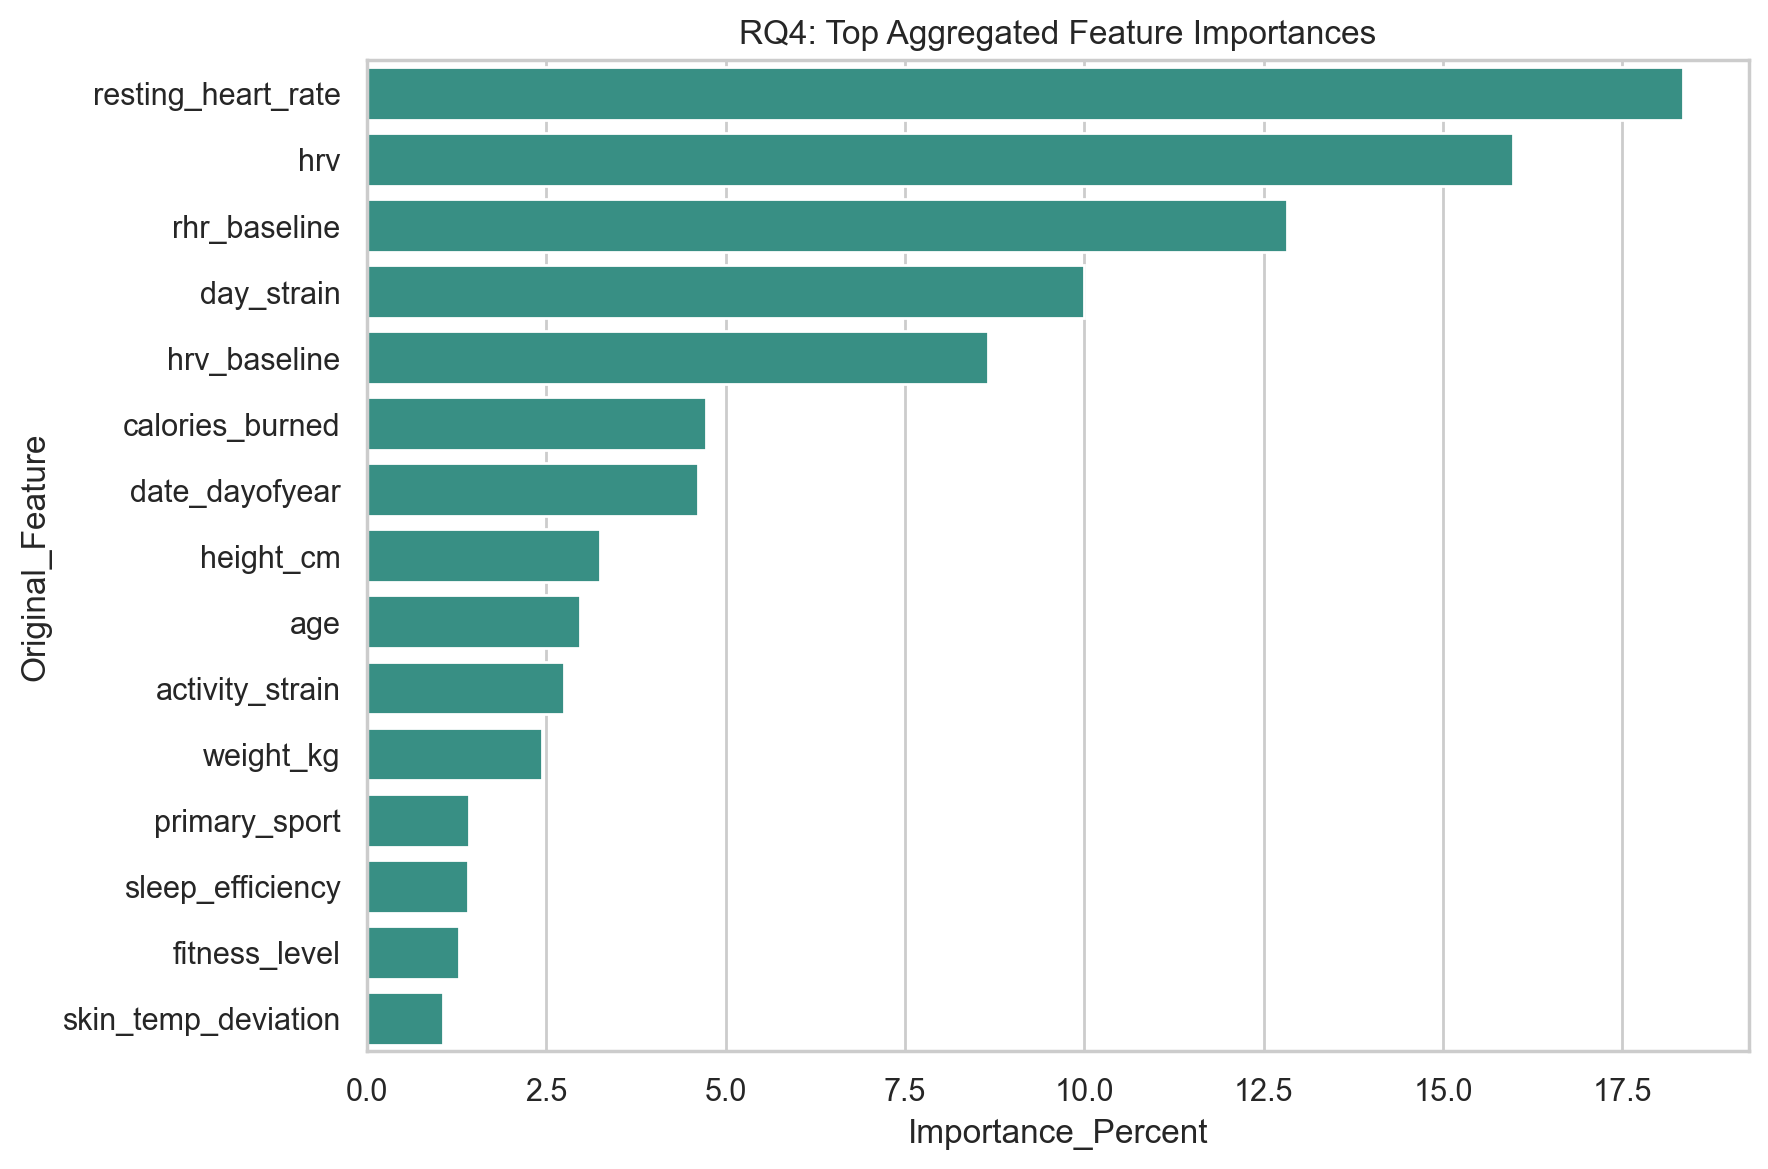
\includegraphics[width=\linewidth]{RQ4_feature_importance_bar.png}
  \caption{Aggregated feature importance showing the dominance of cardiovascular features.}
  \label{fig:rq4}
\end{figure}

\begin{figure}[htbp]
  \centering
  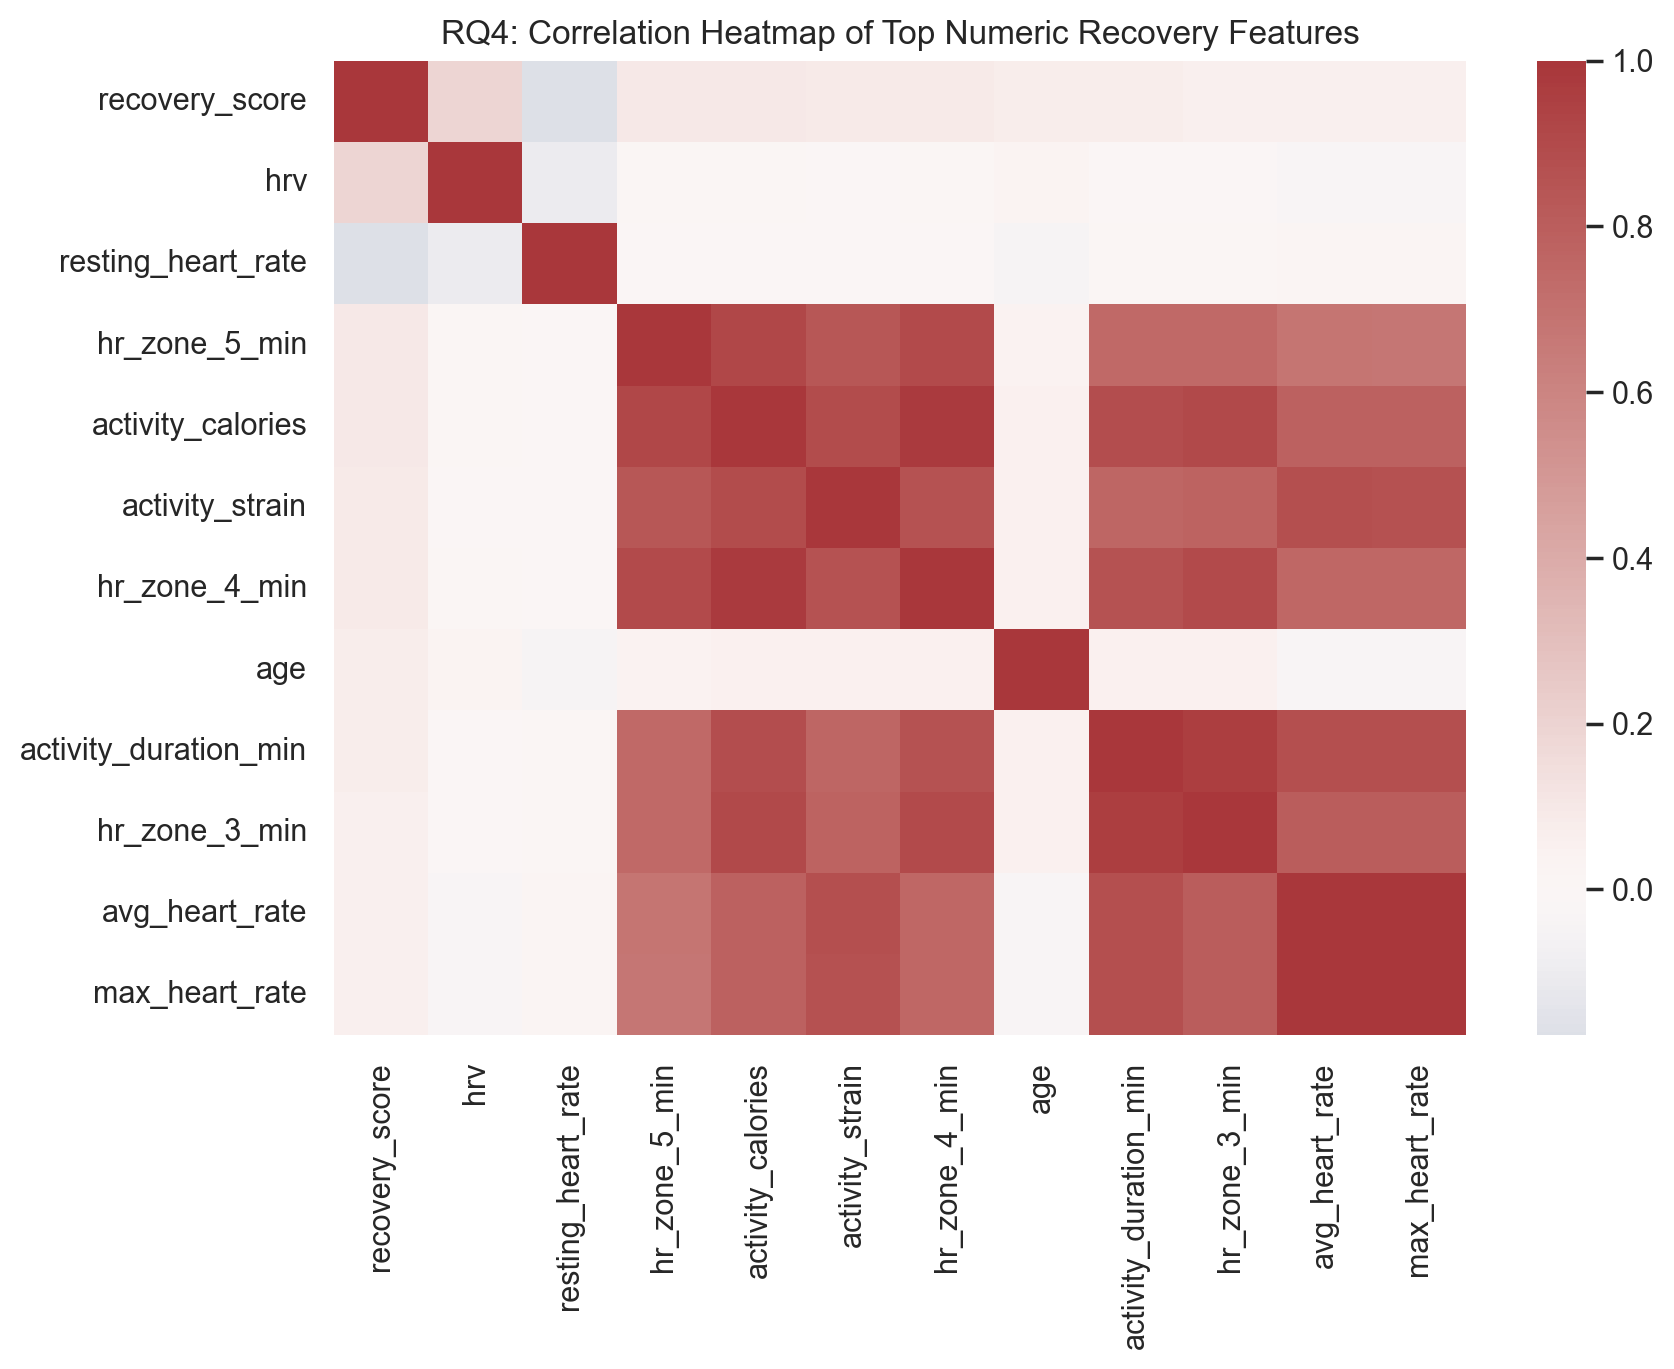
\includegraphics[width=\linewidth]{RQ4_correlation_heatmap.png}
  \caption{Correlation heatmap for important variables used in the project outputs.}
  \label{fig:rq4heat}
\end{figure}

\subsection{RQ5: Stability Across Metrics}
Another useful question is whether the model ranking changes depending on which evaluation metric is used. In this project, the answer was clear: the ranking stayed fully consistent across MAE, RMSE, and \Rsq{}.

\begin{table}[htbp]
\caption{RQ5 Cross-validated Ranking Stability}
\label{tab:rq5}
\centering
\begin{tabular}{lcccc}
\toprule
\textbf{Model} & \textbf{MAE} & \textbf{RMSE} & \textbf{\Rsq} & \textbf{Rank Range} \\
\midrule
Linear Regression & 10.53 & 13.14 & 0.446 & 0 \\
Ridge Regression  & 10.81 & 13.47 & 0.419 & 0 \\
Elastic Net       & 11.11 & 13.79 & 0.390 & 0 \\
XGBoost           & 11.15 & 13.79 & 0.390 & 0 \\
Gradient Boosting & 11.43 & 14.11 & 0.362 & 0 \\
Random Forest     & 11.51 & 14.22 & 0.352 & 0 \\
Decision Tree     & 12.86 & 16.02 & 0.177 & 0 \\
Baseline Mean     & 14.42 & 17.66 & 0.000 & 0 \\
\bottomrule
\end{tabular}
\end{table}

This stability is helpful because it means the model choice does not depend on a metric-specific interpretation. Linear Regression remains the best model no matter whether I focus on average error, squared error, or explained variance.

\begin{figure}[htbp]
  \centering
  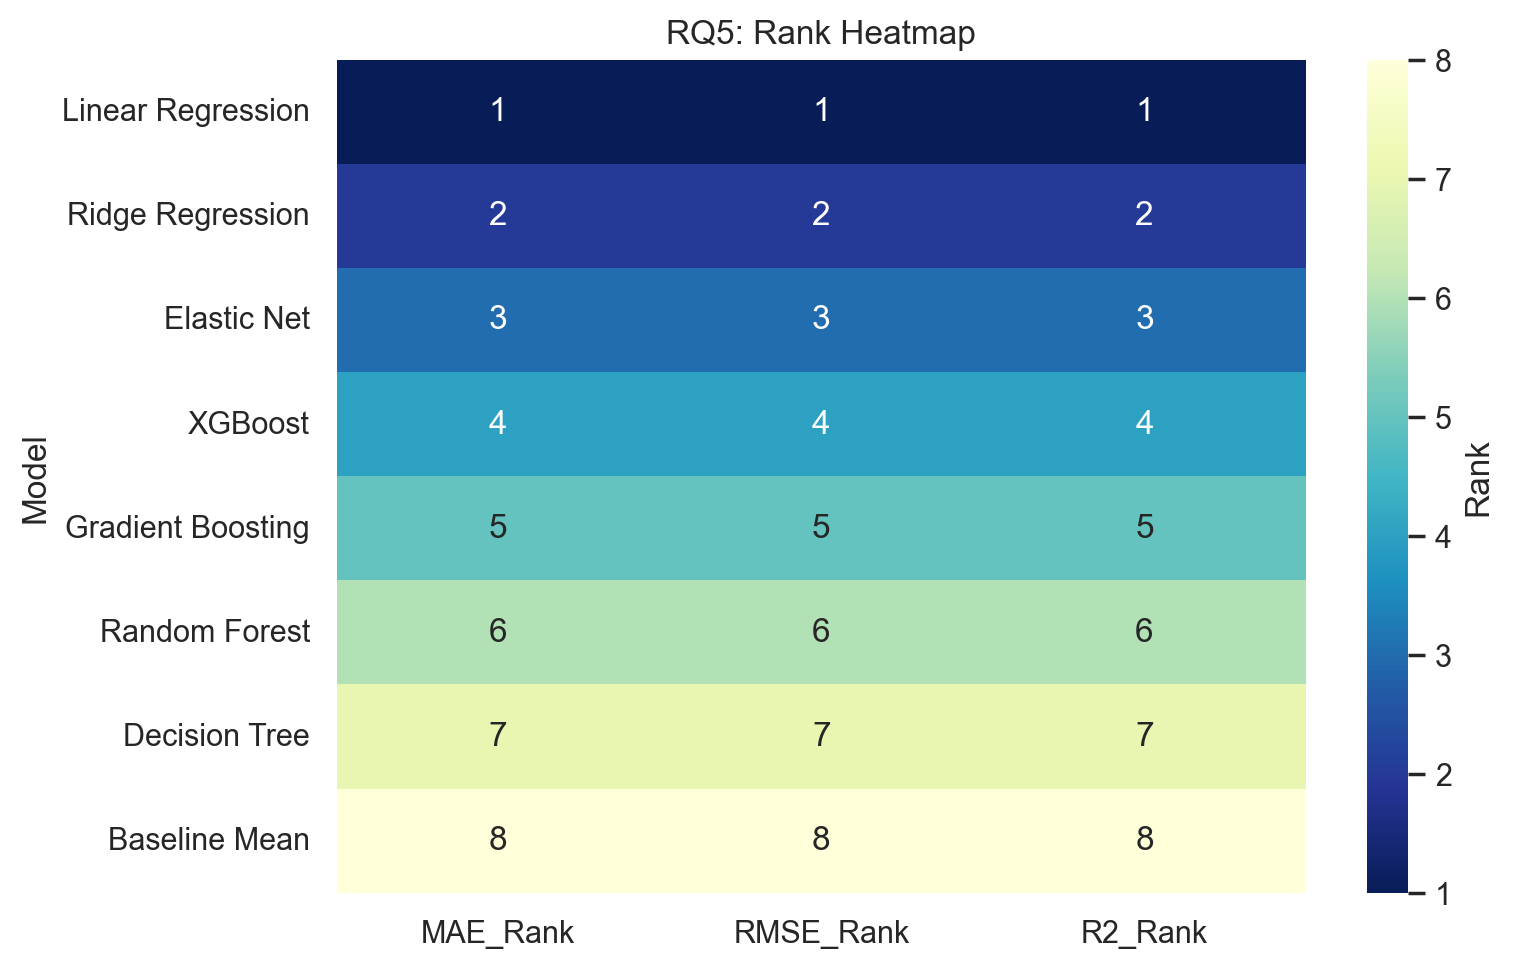
\includegraphics[width=\linewidth]{RQ5_rank_heatmap.png}
  \caption{Heatmap of model ranks across MAE, RMSE, and \Rsq{}.}
  \label{fig:rq5heat}
\end{figure}

\subsection{RQ6: Robustness of the Best Model}
I then tested the best model under more difficult data conditions. The model stayed fairly stable when small noise was added, but it struggled when important values were missing.

\begin{table}[htbp]
\caption{RQ6 Robustness Results for Linear Regression}
\label{tab:robustness}
\centering
\begin{tabular}{lccc}
\toprule
\textbf{Condition} & \textbf{Mean \Rsq} & \textbf{Mean RMSE} & \textbf{Mean MAE} \\
\midrule
Baseline CV          & 0.448 & 13.15 & 10.54 \\
Added numeric noise  & 0.385 & 13.88 & 11.14 \\
Simulated missingness & 0.197 & 15.86 & 12.81 \\
\bottomrule
\end{tabular}
\end{table}

This is an important practical finding. It means the chosen model is usable, but prediction quality depends strongly on data completeness, especially for the key cardiovascular features. In other words, the model can tolerate some noise, but it is much more sensitive when important measurements are missing entirely.

\begin{figure}[htbp]
  \centering
  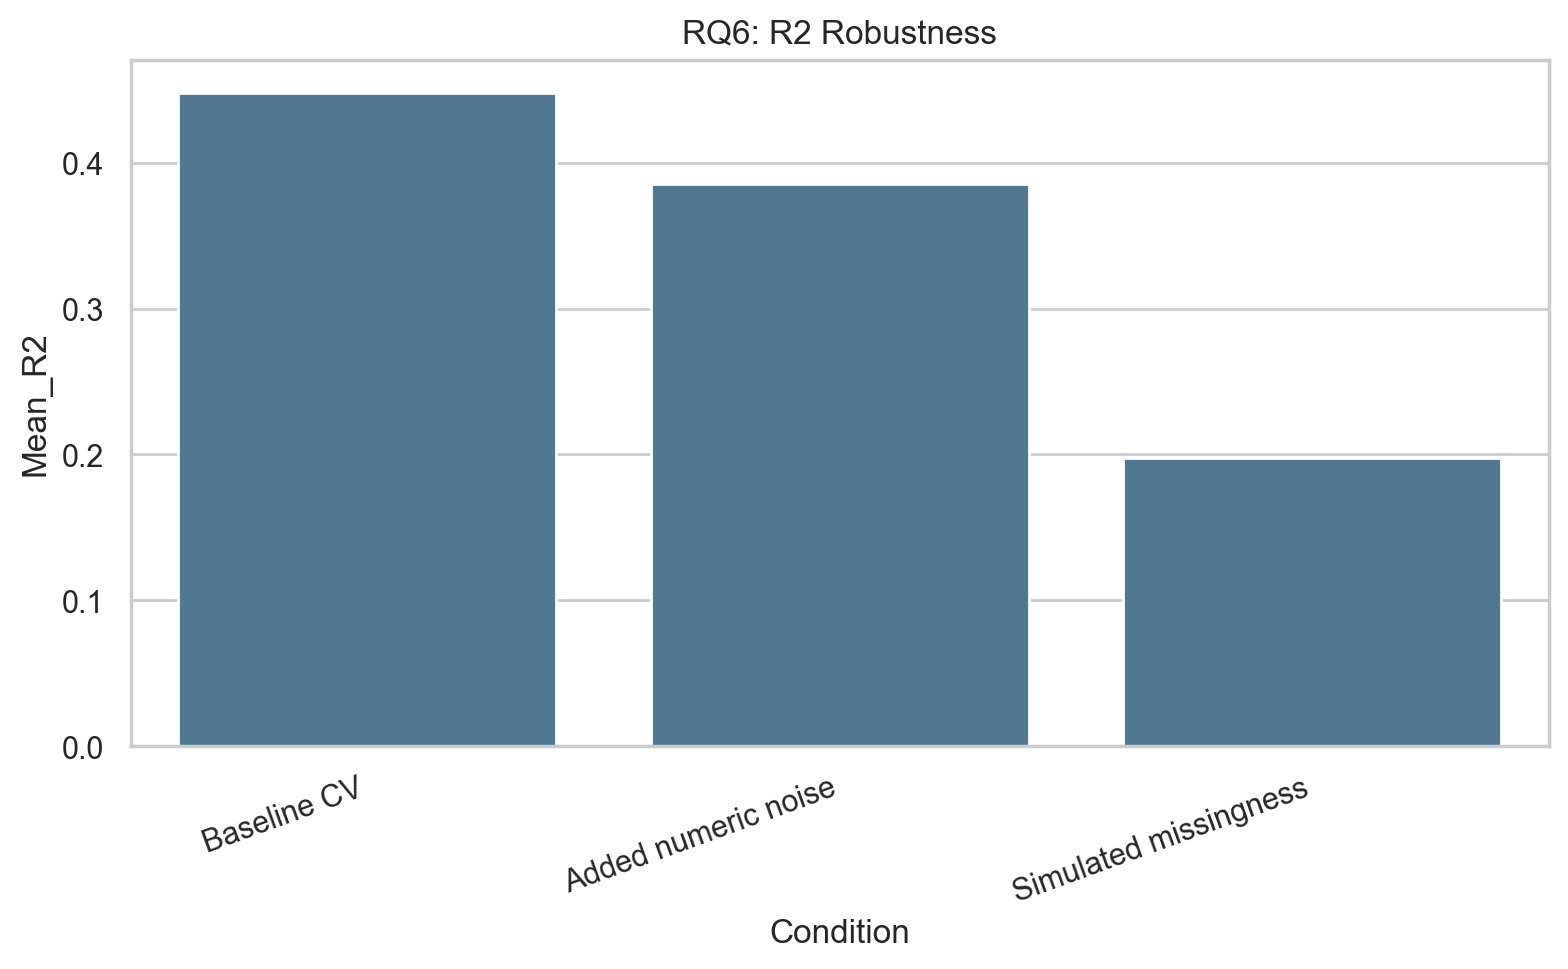
\includegraphics[width=\linewidth]{RQ6_r2_robustness_bar.png}
  \caption{Robustness comparison under clean, noisy, and missing-data conditions.}
  \label{fig:rq6}
\end{figure}

\begin{figure}[htbp]
  \centering
  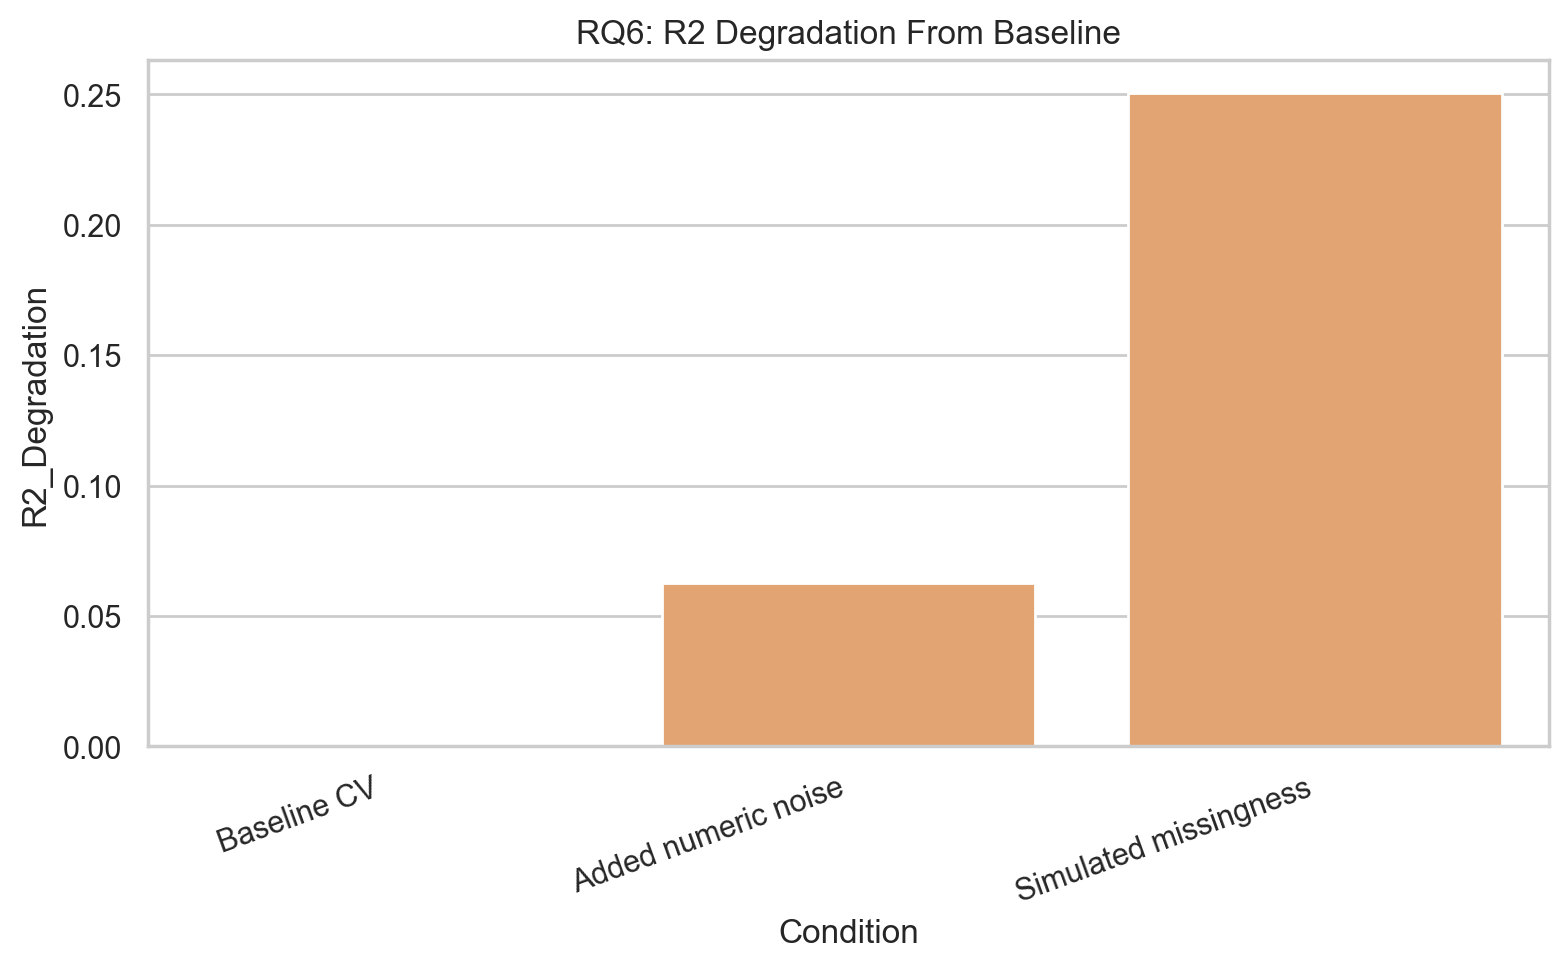
\includegraphics[width=\linewidth]{RQ6_r2_degradation.png}
  \caption{Degradation in \Rsq{} when data quality becomes worse.}
  \label{fig:rq6deg}
\end{figure}

\subsection{RQ7: Final Recommendation}
To make the final recommendation, I did not look only at predictive accuracy. I also included reliability, interpretability, deployment suitability, and computational efficiency. This gave a more practical view of which model would be the best overall choice.

\begin{table}[htbp]
\caption{RQ7 Decision Criteria Weights}
\label{tab:weights}
\centering
\begin{tabular}{lc}
\toprule
\textbf{Criterion} & \textbf{Weight} \\
\midrule
Accuracy & 0.35 \\
Reliability & 0.20 \\
Interpretability & 0.20 \\
Deployment suitability & 0.15 \\
Computational efficiency & 0.10 \\
\bottomrule
\end{tabular}
\end{table}

\begin{table}[htbp]
\caption{RQ7 Final Project Recommendation}
\label{tab:recommendation}
\centering
\begin{tabular}{lc}
\toprule
\textbf{Item} & \textbf{Value} \\
\midrule
Recommended model & Linear Regression \\
Cross-validated \Rsq{} & 0.446 \\
Cross-validated MAE & 10.53 \\
Cross-validated RMSE & 13.14 \\
Weighted decision score & 4.356 \\
Main reason & Best balance of accuracy and simplicity \\
\bottomrule
\end{tabular}
\end{table}

Linear Regression received the highest weighted decision score. This result makes sense because it combined the best predictive performance with strong interpretability and easy deployment. Ridge Regression was also a good option, but Linear Regression still stayed ahead in the final comparison.

\begin{figure}[htbp]
  \centering
  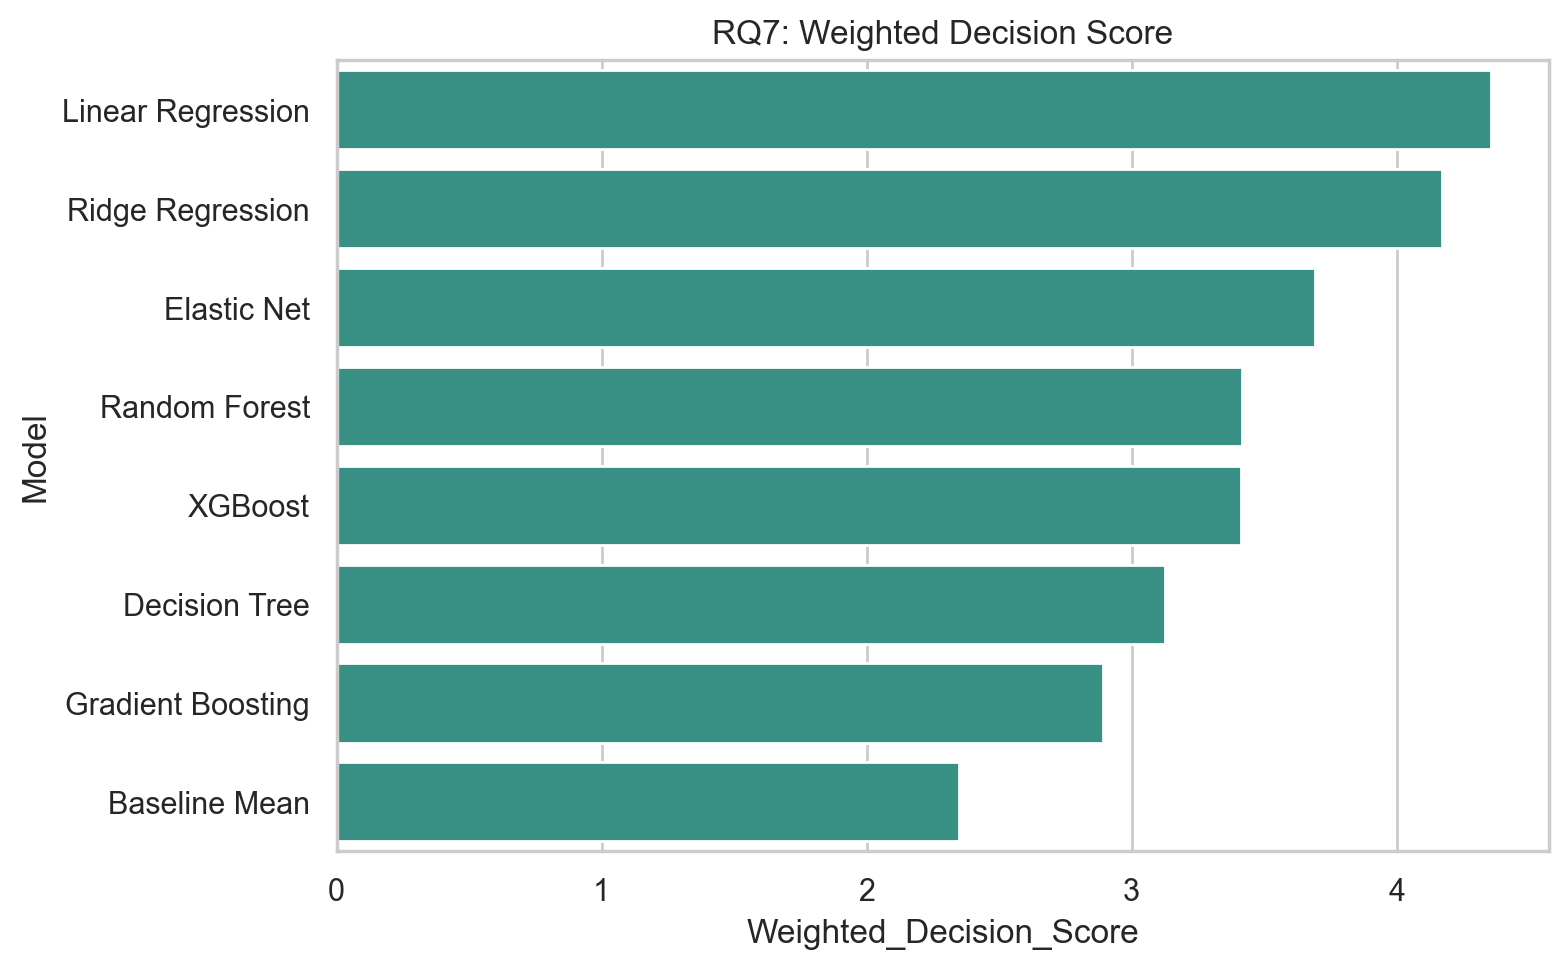
\includegraphics[width=\linewidth]{RQ7_weighted_decision_score.png}
  \caption{Weighted decision score used for the final model recommendation.}
  \label{fig:rq7}
\end{figure}

\begin{figure}[htbp]
  \centering
  
\includegraphics[width=\linewidth]{RQ7_decision_matrix_heatmap.png}
  \caption{Heatmap of the decision matrix used in the final recommendation step.}
  \label{fig:rq7heat}
\end{figure}

\section{Conclusion}
This project shows that WHOOP recovery score prediction can be handled effectively with a simple supervised learning model. Across both hold-out and cross-validated evaluation, Linear Regression gave the best overall result. The model remained easy to explain, fast to run, and practical for deployment, which made it a stronger choice than the more complex ensemble alternatives in this specific dataset.

The feature analysis showed that the most useful predictors were resting heart rate, HRV, and their baseline values. This is meaningful because it connects the machine learning results to the physiological idea of recovery. The preprocessing experiments also showed that a simple numeric-only pipeline with median imputation was already enough to achieve strong results, which reduced the need for unnecessary complexity.

The robustness analysis added an important practical lesson. The best model was reasonably stable under small numeric noise, but it was much more sensitive to missing values. This means that, in practice, data completeness matters a lot, especially for the key cardiovascular features.

Overall, my results suggest that a simpler model is the better choice for this dataset. It provides solid predictive performance while staying easier to interpret and easier to deploy than more complicated methods. The report, code, tables, and figures are aligned because all presented numbers come directly from the outputs generated by the implemented pipeline.

\section*{Acknowledgement}
This report was prepared for the supervised learning assignment under the guidance of Prof. Raja Hashim Ali.

\begin{thebibliography}{9}
\bibitem{plews2013heart}
D.~J. Plews, P.~B. Laursen, J.~Stanley, A.~E. Kilding, and M.~Buchheit,
``Training adaptation and heart rate variability in elite endurance athletes,''
\textit{Sports Medicine}, vol.~43, no.~9, pp.~773--781, 2013.

\bibitem{bellenger2016monitoring}
C.~R. Bellenger, R.~L. Thomson, J.~D. Buckley, M.~Davison, P.~W. Robertson, and J.~T. Fuller,
``Monitoring athletic training status through autonomic heart rate regulation,''
\textit{Sports Medicine}, vol.~46, no.~10, pp.~1461--1486, 2016.

\bibitem{whoop2023methodology}
WHOOP, Inc.,
``WHOOP recovery: Understanding your recovery score,''
2023. [Online]. Available: \url{https://www.whoop.com/thelocker/how-whoop-calculates-recovery/}

\bibitem{sklearn}
F. Pedregosa et al.,
``Scikit-learn: Machine learning in Python,''
\textit{Journal of Machine Learning Research}, vol.~12, pp.~2825--2830, 2011.

\bibitem{chen2016xgboost}
T. Chen and C. Guestrin,
``XGBoost: A scalable tree boosting system,''
in \textit{Proceedings of the 22nd ACM SIGKDD International Conference on Knowledge Discovery and Data Mining}, 2016, pp.~785--794.

\bibitem{kaggle_whoop}
L. Gedipudi,
``WHOOP Fitness Dataset,''
Kaggle, 2024. [Online]. Available: \url{https://www.kaggle.com/datasets/likithagedipudi/whoop-fitness-dataset}
\end{thebibliography}

\balance
\end{document}
